\documentclass[handout]{beamer}

\usepackage[utf8]{inputenc}
\usepackage[english,russian]{babel}
\usepackage{listings}

%\ifx\pdftexversion\undefined
%\usepackage[dvips]{graphicx}
%\else
%\usepackage[pdftex]{graphicx}
%\DeclareGraphicsRule{*}{mps}{*}{}
%#\fi

\definecolor{javared}{rgb}{0.6,0,0} % for strings
\definecolor{javagreen}{rgb}{0.25,0.5,0.35} % comments
\definecolor{javapurple}{rgb}{0.5,0,0.35} % keywords
\definecolor{javadocblue}{rgb}{0.25,0.35,0.75} % javadoc
 
\lstset{language=Java,
basicstyle=\footnotesize\ttfamily,
keywordstyle=\color{javapurple}\bfseries,
stringstyle=\color{javared},
commentstyle=\color{javagreen},
morecomment=[s][\color{javadocblue}]{/**}{*/},
stepnumber=2,
numbersep=10pt,
tabsize=4,
showspaces=false,
showstringspaces=false}


\title{Паттерн Observer, MVC}
\author{Есилевич Александр}

\begin{document}

\maketitle


\begin{frame}[fragile]
\frametitle{Редактирование свойств фигур}
\begin{itemize}
\item Пользователь выбирает фигуру
\item На панели свойств отображаются свойства фигуры
\item При изменении свойств в панели меняется фигура
\item При изменении фигуры мышью меняются свойства в панели
\end{itemize}
\end{frame}


\begin{frame}[fragile]
\frametitle{Вопросы реализации}
\begin{itemize}
\item Теперь у каждой фигуры есть состояние (набор координат, свойства)
      и несколько представлений этого состояния
\item Как отделить состояние фигуры от её представления?
\item Как добиться того, чтобы можно было легко добавлять новые представления?
\end{itemize}
\end{frame}


\begin{frame}[fragile]
\frametitle{Реализация}
\begin{itemize}
\item Вынесем состояние каждой фигуры в отдельный класс ''модели'': \lstinline{LineModel},
      \lstinline{CircleModel}, \lstinline{RectangleModel};
\item Для каждой фигуры определим определим интерфейс ''наблюдателя'' за состоянием
      фигуры: \lstinline{LineObserver}, \lstinline{CircleObserver}, \lstinline{RectangleObserver};
\item Добавим классы моделей методы для регистрации наблюдателей за состоянием модели;
\item При изменении состояния модели будем оповещать об изменении всех наблюдателей.
\end{itemize}
\end{frame}


\begin{frame}[fragile]
\frametitle{Интерфейс LineObserver}
\begin{lstlisting}
public interface LineObserver {
    void update();
};
\end{lstlisting}
\end{frame}


\begin{frame}[fragile]
\frametitle{Класс LineModel}
\begin{lstlisting}
public class LineModel {
    public void attach(LineObserver o) {
        observers.add(o); }
    	
    public void detach(LineObserver o) {
        observers.remove(o); }
        
    public void notify() {
    	for each o in observers: o.notify(); }
    	
    ...
\end{lstlisting}
\end{frame}


\begin{frame}[fragile]
\frametitle{Класс LineModel}
\begin{lstlisting}
    ...
    
    public Point getStart() {
        return new Point(x1, y1); }
        
    public void setStart(int px1, int py1) {
        x1 = px1; y1 = py1; notify(); }
        
    private int x1, x2, y1, y2;
    private LineObserverList observers;
};
\end{lstlisting}
\end{frame}


\begin{frame}[fragile]
\frametitle{Класс Line}
\begin{lstlisting}
public class Line extends Shape implements LineObserver {
    public LineObserver(LineModel mdl) {
        model = mdl; }
        
    public Point getStart() { return model.getStart(); }
    public Point setStart(Point p) { model.setStart(p); }
    
    public void notify() {
        // notify scene about changes
    }
    
    private LineModel model;
};
\end{lstlisting}
\end{frame}


\begin{frame}[fragile]
\frametitle{Класс LinePanel}
\begin{lstlisting}
public class LinePanel extends SystemComponent
                       implements LineObserver {
		
    public LinePanel(LineModel mdl) {
        model = mdl;
        // make edit boxes
    }
        
    public void notify() {
        Point start = model.getStart();
        Point end = mode.getEnd();
        
        startX.setText(Integer.toString(start.x));
        startY.setText(Integer.toString(start.y));
        endX.setText(Integer.toString(end.x));
        endY.setText(Integer.toString(end.y));
    }
    
    private LineModel model;
    private SystemEditBox startX, startY, endX, endY;
};
\end{lstlisting}
\end{frame}


\begin{frame}[fragile]
\frametitle{Диаграмма классов}
\begin{center}
\includegraphics{line_observer.mps}
\end{center}
\end{frame}


\begin{frame}[fragile]
\frametitle{Паттерн Observer}
Определяет зависимость ''один ко многим'' таким образом, что при изменении состояния
одного объекта все зависящие от него оповещаются об этом и автоматически обновляются.
\end{frame}


\begin{frame}[fragile]
\frametitle{Применимость}
\begin{itemize}
\item у абстракции есть два аспекта, один из которых зависит от другого
\item при модификации одного аспекта требуется изменить другие
\item один объект должен оповещать других, не зная о конкретных оповещаемых объектах
\end{itemize}
\end{frame}



\begin{frame}[fragile]
\frametitle{Диаграмма классов}
\begin{center}
\includegraphics{observer.mps}
\end{center}
\end{frame}



\begin{frame}[fragile]
\frametitle{Результаты}
\begin{itemize}
\item минимизация связей между субъектом и наблюдателями
\item поддержка широковещательных коммуникаций
\item сложность отслеживания эффектов от изменения субъекта
\end{itemize}
\end{frame}


\begin{frame}[fragile]
\frametitle{MVC -- Model-View-Controller}
\begin{center}
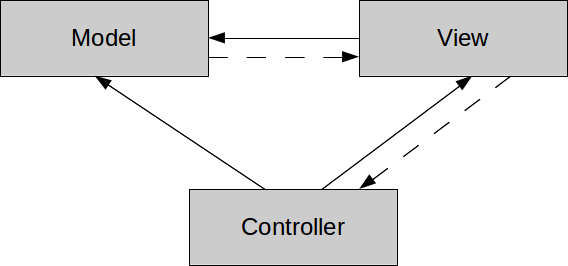
\includegraphics[scale=0.4]{mvc.png}
\end{center}
\end{frame}


\begin{frame}[fragile]
\frametitle{Участники}
\begin{itemize}
\item Model - модель, хранит состояние абстракции
\item View - представление абстракции
\item Controller - обработчик событий, возникающих в абстракции
\end{itemize}
\end{frame}


\begin{frame}[fragile]
\frametitle{Отношения между участниками}
\begin{itemize}
\item Model-View -- паттерн Observer
\item View-Controller -- паттерн Strategy
\item Controller-Model -- использование/ассоциация
\end{itemize}
\end{frame}



\end{document}
